\documentclass[a4paper]{article}
\usepackage[utf8]{inputenc}
\usepackage[russian,english]{babel}
\usepackage[T2A]{fontenc}
\usepackage[left=10mm, top=20mm, right=18mm, bottom=15mm, footskip=10mm]{geometry}
\usepackage{indentfirst}
\usepackage{amsmath,amssymb}
\usepackage{mathastext} 
\usepackage[italicdiff]{physics}
\usepackage{graphicx}
\usepackage{caption}
\usepackage{float}
\usepackage{caption}
\renewcommand{\thefootnote}{\fnsymbol{footnote}}
\usepackage{tablefootnote}
\usepackage{footmisc}
\usepackage{textcomp}
\usepackage{multicol}
\usepackage{multirow}
\usepackage[parfill]{parskip}
\usepackage{makecell}
\usepackage{array}  
\usepackage{siunitx}
\usepackage{booktabs}
\sisetup{
    exponent-product = \cdot,
    per-mode = symbol,
    separate-uncertainty = true,
    uncertainty-separator = \,
}
\renewcommand\cellalign{cc} 
\renewcommand\cellgape{\Gape[2pt]} 
\usepackage[utf8]{inputenc}\newcommand{\approxtext}[1]{\ensuremath{\stackrel{\text{#1}}{\approx}}}
\usepackage[colorlinks=true, urlcolor=blue, linkcolor=blue, citecolor=blue]{hyperref}
\graphicspath{{images/}}
\DeclareGraphicsExtensions{.pdf,.png,.jpg}
\usepackage{wrapfig}
\captionsetup{labelformat=empty}
\usepackage{caption}
\captionsetup[figure]{name=Рисунок}
\captionsetup[table]{name=Таблица}
%\usepackage{newtxtext,newtxmath} 
\title{\textbf{Отчет о выполнении лабораторной работы 3.7.3}}
\date{}
\author{Котляров Михаил, Б01-402}

\begin{document}

\maketitle
	
\section{Введение}

\subsubsection*{Цель работы}
Ознакомиться с теорией распространения электрических сигналов вдоль длинной линии; измерить амплитудно-частотные и фазо-частотные характеристики коаксиальной линии; определить волновые характеристики такой линии; изучить распределение амплитуды колебаний сигнала по длине линии.

\subsubsection*{Оборудование}
\begin{itemize}
    \item Осциллограф АКТАКОМ ADS-6142H
    \item Генератор АКИП 3420/1
    \item Бухта с коаксиальным кабелем РК 50-4-11
    \item Схематический блок "модель длинной линии"
    \item Магазин сопротивлений Р33
    \item Соединительные провода
\end{itemize}

\subsection{Теоретическая часть}

Длинной линией называется линия передачи, геометрическая длина которой сравнима или превышает длину волны передаваемого сигнала. В данной работе исследуется коаксиальный кабель, состоящий из двух коаксиальных проводников с радиусами $r_1$ и $r_2$, заполненных диэлектриком с параметрами $\varepsilon$ и $\mu$.

\begin{figure}[h]
    \centering
    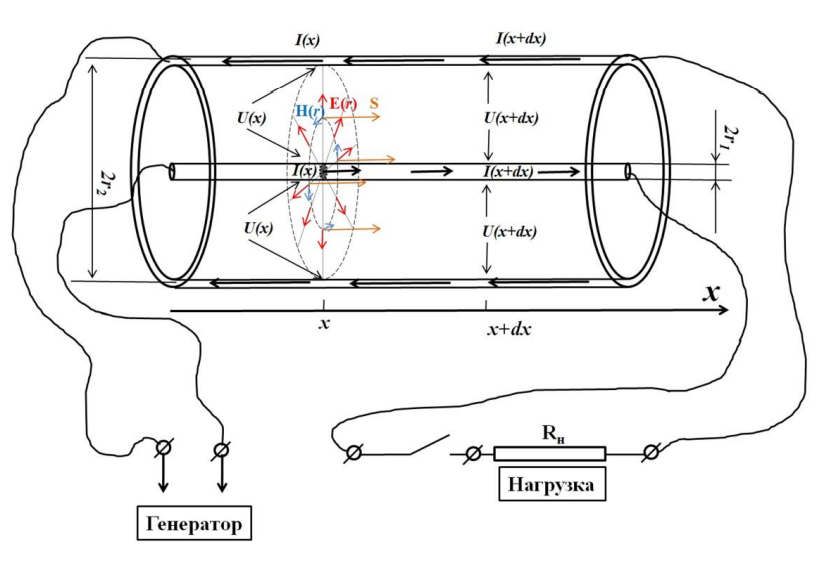
\includegraphics[scale=0.8]{Pictures/cabel.png}
    \caption{Схема коаксиального кабеля}
\end{figure}

Распространение сигналов в длинной линии описывается телеграфными уравнениями:

\begin{equation}
\begin{cases}
    \dfrac{\partial I}{\partial x} = -C_x \dfrac{\partial U}{\partial t} \\
    \dfrac{\partial U}{\partial x} = -\dfrac{L_x}{c^2} \dfrac{\partial I}{\partial t} - R_x I
\end{cases}
\end{equation}

где $L_x$, $C_x$, $R_x$ -- погонные индуктивность, ёмкость и сопротивление линии.

Для коаксиального кабеля погонные параметры выражаются через геометрию и свойства материалов:

\begin{equation}
L_x = 2\mu\ln\left(\frac{r_2}{r_1}\right), \quad 
C_x = \frac{\varepsilon}{2\ln(r_2/r_1)}
\end{equation}

Волновое уравнение для напряжения имеет вид:

\begin{equation}
\frac{\partial^2 U}{\partial t^2} - V_{\phi}^2 \frac{\partial^2 U}{\partial x^2} + \gamma \frac{\partial U}{\partial t} = 0
\end{equation}

где $V_{\phi} = \dfrac{c}{\sqrt{L_x C_x}} = \dfrac{c}{\sqrt{\varepsilon\mu}}$ -- фазовая скорость, $\gamma = R_x C_x V_{\phi}^2$ -- декремент затухания.

Решение волнового уравнения ищется в виде:

\begin{equation}
U(x,t) = U_0 e^{-i\omega t} e^{(-\alpha + ik)x}
\end{equation}

где $\alpha$ -- коэффициент затухания, $k$ -- волновое число.

Волновое сопротивление линии определяется как:

\begin{equation}
Z = \frac{1}{c}\sqrt{\frac{L_x}{C_x}}
\end{equation}

При согласованной нагрузке $R_0 = Z$ отраженная волна отсутствует.

Экспериментально определяемые параметры:

\begin{equation}
\alpha = \frac{1}{l}\ln\left(\frac{U_0}{U_\text{н}}\right), \quad 
k = \frac{\Delta \varphi}{l}
\end{equation}

\subsection{Экспериментальная установка}

\begin{figure}[h]
    \centering
    
\includegraphics[scale=0.8]{Pictures/ustanovka.png}
    \caption{Схема экспериментальной установки}
\end{figure}

Для исследования длинной линии собираем схему, содержащую:
\begin{itemize}
    \item Генератор сигналов АКИП-3420/1
    \item Осциллограф АКТАКОМ ADS-6142H  
    \item Коаксиальный кабель РК-50-4-11 длиной $l$
    \item Нагрузочные сопротивления
\end{itemize}

Сигнал от генератора подается на вход линии и одновременно на канал CH1 осциллографа. С выхода линии сигнал поступает на канал CH2 осциллографа. Измеряем амплитуды входного и выходного сигналов, а также фазовый сдвиг между ними.

\subsection{Методика измерений}

\begin{enumerate}
    \item Измеряем резонансные частоты для различных типов сигналов и нагрузок
    \item Снимаем амплитудно-частотную и фазо-частотную характеристики
    \item Определяем погонные параметры линии $L_x$ и $C_x$
    \item Рассчитываем диэлектрическую проницаемость $\varepsilon$ и магнитную восприимчивость $\mu$
    \item Определяем удельную проводимость $\sigma$ материала проводников
\end{enumerate}



\section{Выполнение}

Параметры кабеля:
\begin{itemize}
\item Модель: Eltros PK 50-4-11
\item Длина: $l = 5052,7$ см
\item $r_1 = 0,137 \pm 0,002$ см, $r_2 = 0,46 \pm 0,01$ см.
\end{itemize}

\subsection*{I. Оценка фазовой и групповой скорости}

\begin{enumerate}

\item В первом задании эксперимента измерим резонансные частоты коаксиальной линии для различных типов сигналов и режимов нагрузки:

\begin{itemize}
    \item Синусоидальный сигнал с согласованной нагрузкой 50 Ом
    \item Синусоидальный сигнал без нагрузки (холостой ход)
    \item Прямоугольные импульсы с согласованной нагрузкой 50 Ом
    \item Прямоугольные импульсы без нагрузки
\end{itemize}

Для каждого режима определим несколько последовательных резонансных частот, соответствующих условию, когда фазовый набег вдоль линии кратен $2\pi$. 

\begin{table}[h!]
    \centering
    \begin{tabular}{|c|c|c|c|c|}
        \hline
        $n$ & $\nu_{\text{синус с нагр}}$, МГц & $\nu_{\text{синус без нагр}}$, МГц & $\nu_{\text{прям с нагр}}$, МГц & $\nu_{\text{прям без нагр}}$, МГц \\ \hline
        1 & 3,94 & 3,80 & 3,97 & 3,98 \\ \hline
        2 & 7,90 & 8,02 & 7,95 & 7,94 \\ \hline
        3 & 11,91 & 12,05 & 11,94 & 11,90 \\ \hline
        4 & 15,89 & 16,01 & 15,92 & 15,87 \\ \hline
        5 & 19,88 & 20,01 & 19,91 & 19,85 \\ \hline
        6 & 23,89 & 23,99 & 23,88 & 23,82 \\ \hline
        7 & 27,87 & 27,95 & 27,84 & 27,77 \\ \hline
    \end{tabular}
    \caption{Таблица 1. Резонансные частоты для различных типов сигналов и нагрузок}
    \label{tab:resonance_freq}
\end{table}

\item По МНК построим линейную аппроксимацию зависимости резонансной частоты от номера резонанса\\ $\nu(n) = k \cdot n$.
\clearpage
 \begin{figure}[h]
      \center{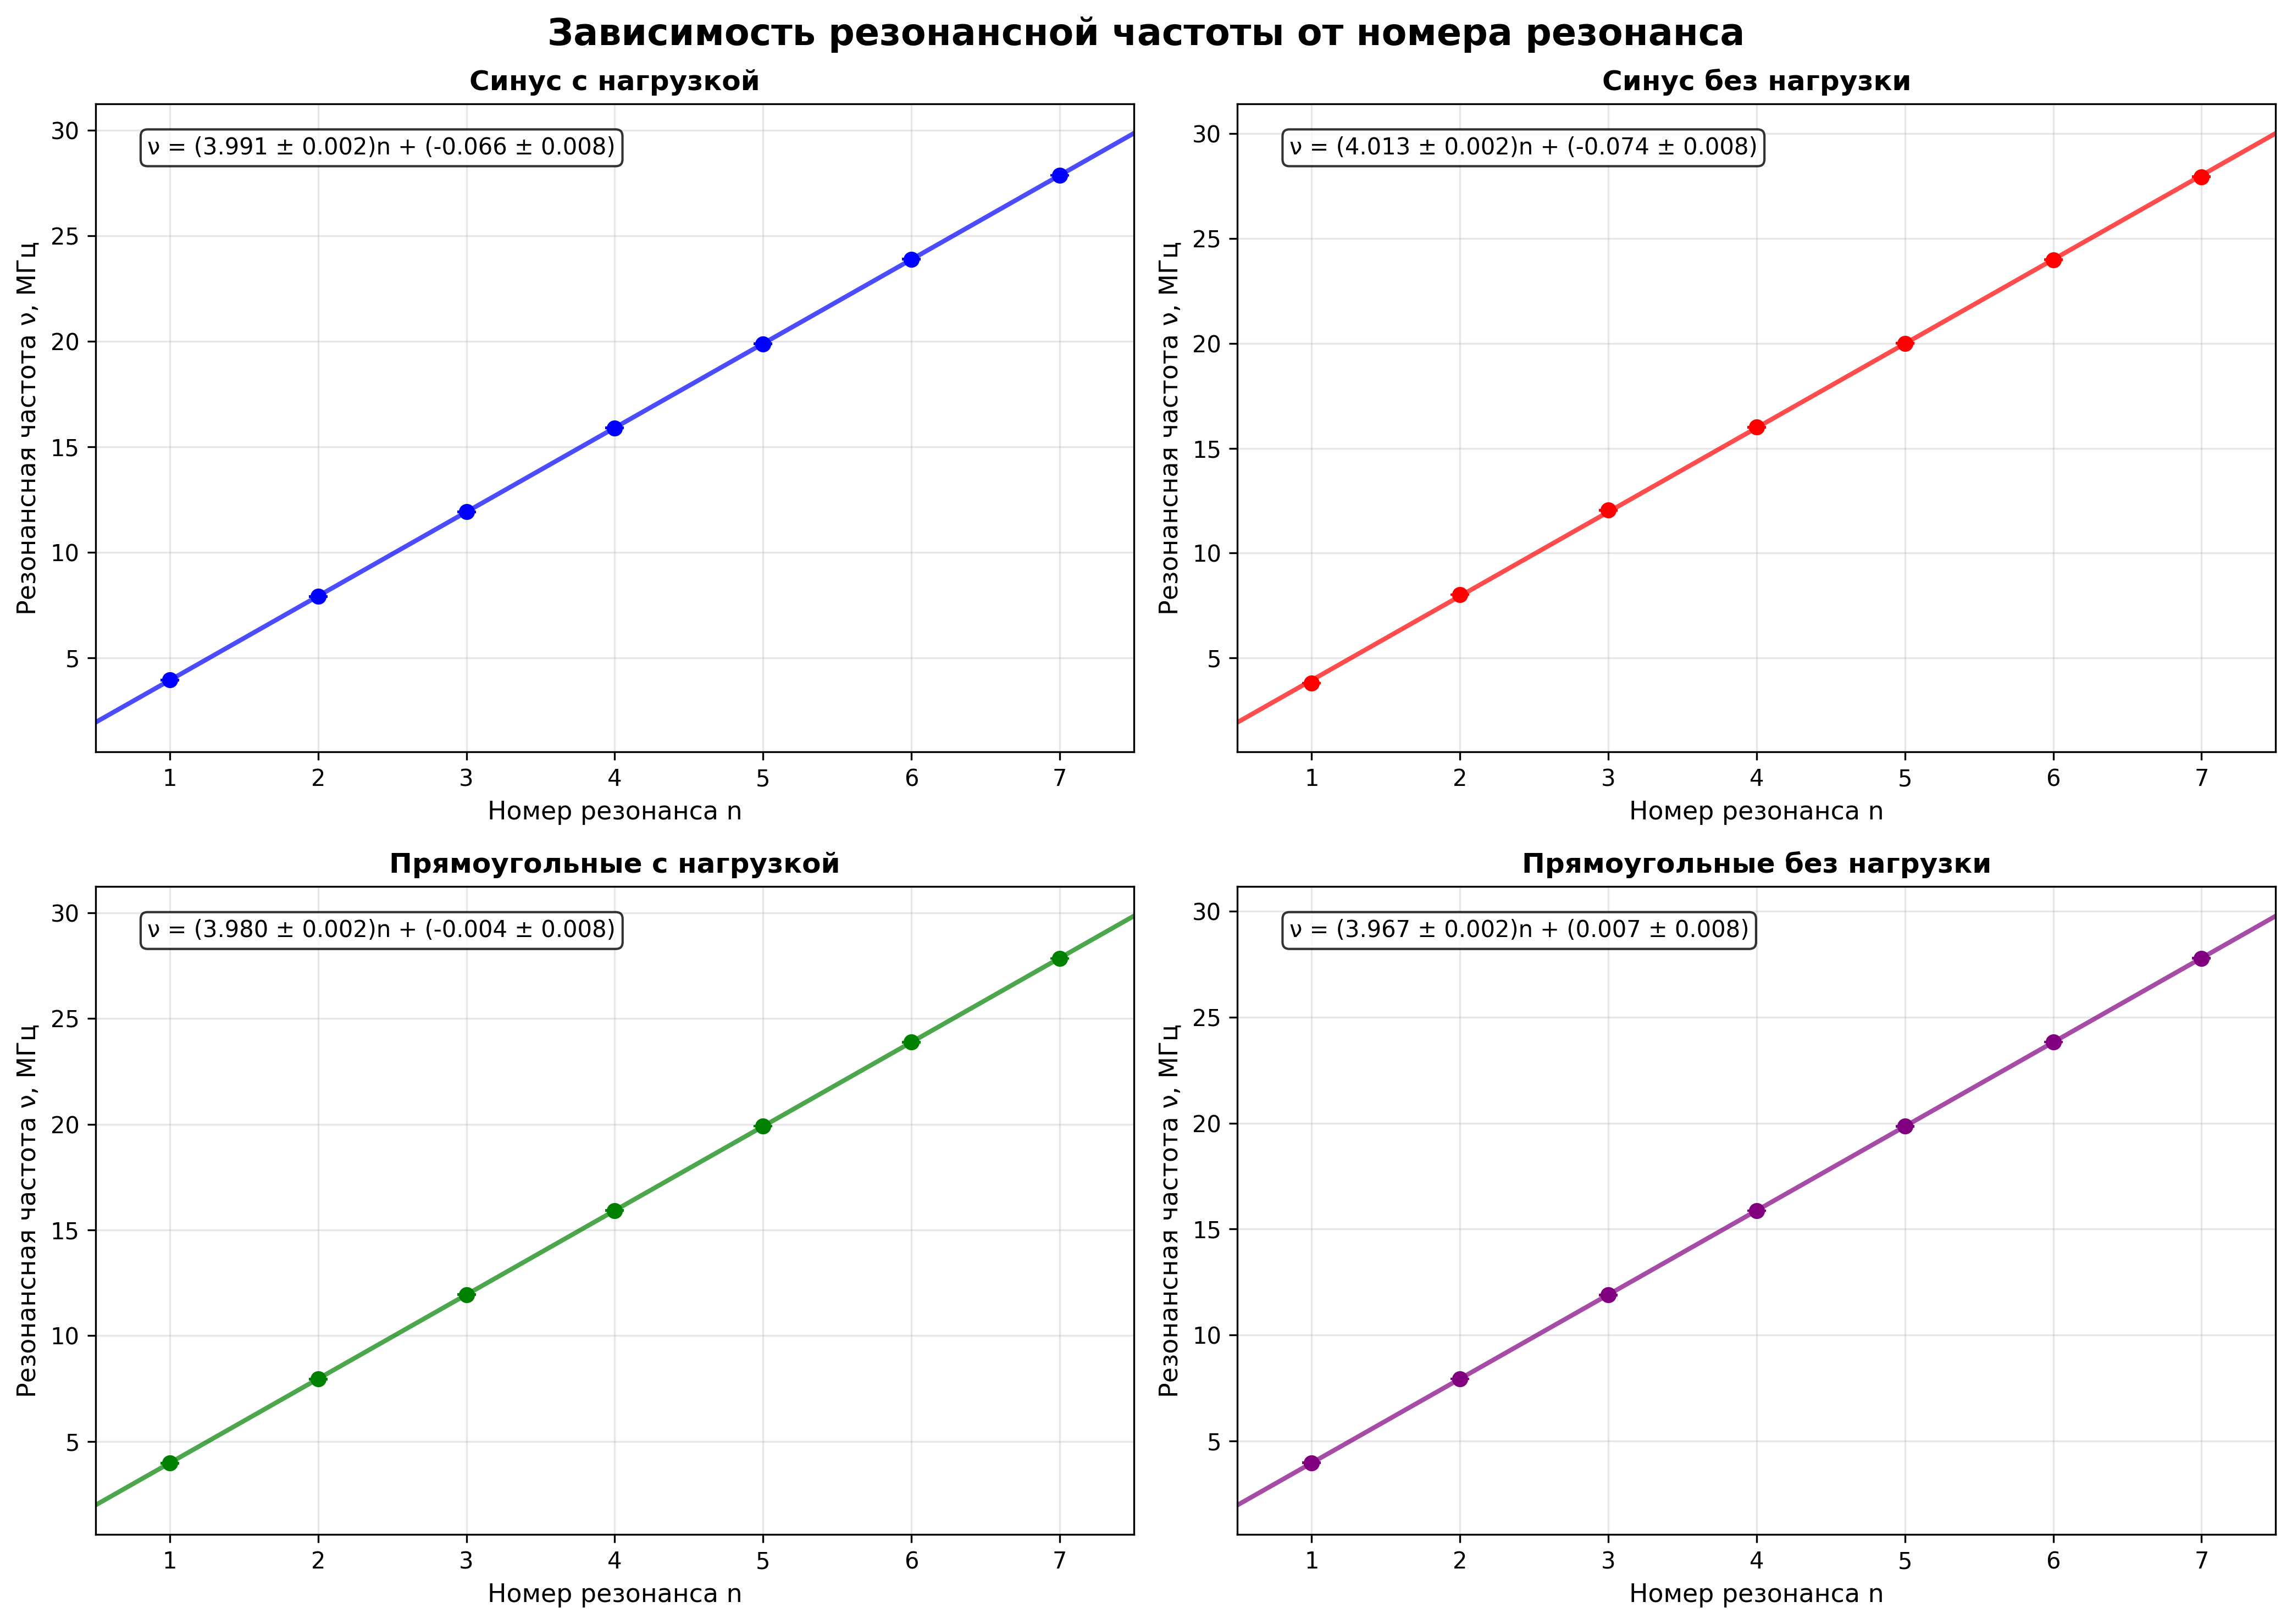
\includegraphics[width=1\textwidth]{Graphics/nu_vs_n.png}}
      \caption{График 1. Зависимость резонансной частоты от номера}
\end{figure}

Резонансные частоты соответствуют сдвигу фаз, кратному $2\pi$, поэтому для каждой такой частоты справедливо из формулы (6): $k=\frac{2\pi (n+n_0)}{l}$.  
\begin{equation}
 		\nu_n=\frac{V_\text{ф}}{l}(n+n_0)
	\end{equation}
В случае прямоугольных импульсов резонансные частоты соответствуют ситуации, когда
	временной сдвиг между сигналом на входе и выходе длинной линии кратен периоду
	повторений импульсов, т.е $\Delta t = \frac{1}{\nu_n}(n+n_0)$. Временной сдвиг задаётся соотношением
	$\Delta t=\frac{l}{V_\text{гр}}$, где $V_\text{гр}$ -- групповая скорость. Тогда в случае резонанса получим.
	\begin{equation}
		\nu_n=\frac{V_\text{гр}}{l}(n+n_0)
	\end{equation}

Наклон полученных прямых позволяет определить скорость распространения волн в кабеле:
 \clearpage
\begin{table}[h!]
    \centering
    \begin{tabular}{|c|c|c|c|c|}
        \hline
        Тип сигнала & $k \pm \sigma_k$, МГц & $\varepsilon_k$, \% & $V_{\Phi} \pm \sigma_{V_{\Phi}}$, $10^{10}$ см/с  \\ \hline
        Синус с нагр. & $3,9907 \pm 0,0019$ & 0,0476 & $2,016 \pm 0,0096$ \\ \hline
        Синус без нагр. & $4,0125 \pm 0,0019$ & 0,0474 & $2,027 \pm 0,0096$  \\ \hline
        Прям. с нагр. & $3,98 \pm 0,0019$ & 0,0477 & $2,011 \pm 0,0096$  \\ \hline
        Прям. без нагр. & $3,9671 \pm 0,0019$ & 0,0479 & $2,004 \pm 0,0096$ \\ \hline
    \end{tabular}
    \caption{Таблица 2. Параметры линейной аппроксимации и фазовые скорости}
    \label{tab:velocity_params}
\end{table}

\item Рассчитанные значения скоростей распространения для всех четырех режимов оказались близкими друг к другу и составили приблизительно $(2,01-2,03) \cdot 10^{10}$ см/с. Совпадение фазовой и групповой скоростей указывает на \textbf{отсутствие значительной дисперсии} в исследуемом коаксиальном кабеле в диапазоне частот 3-28 МГц.

Относительная погрешность определения коэффициента наклона $k$ не превышает 0,05\%, что свидетельствует о высокой точности проведенных измерений и надежности полученных результатов.

\subsection*{II. Измерение АЧХ и ФЧХ}

    \item Установим синусоидальный сигнал амплитудой 1 В с согласованной нагрузкой. Измерим амплитуды и фазовые сдвиги для частот от 1 до 40 МГц.
\begin{table}[h!]
    \centering
    \begin{tabular}{|c|c|c|c|c|}
        \hline
        $\nu$, МГц & $\Delta x$, нс & $\Delta \varphi \pm \sigma_{\Delta \varphi}$, рад & $U_{\text{вх}}$, В & $U_{\text{вых}}$, В \\ \hline
        1,0 & 252,0 & $1,58 \pm 0,01$ & 27,2 & 25,2 \\ \hline
        3,5 & 254,0 & $5,59 \pm 0,04$ & 26,8 & 24,2 \\ \hline
        6,0 & 252,7 & $9,53 \pm 0,08$ & 26,8 & 23,6 \\ \hline
        8,5 & 252,9 & $13,51 \pm 0,11$ & 26,8 & 22,44 \\ \hline
        11,0 & 252,2 & $17,43 \pm 0,14$ & 27,26 & 22,04 \\ \hline
        13,5 & 292,6 & $24,82 \pm 0,17$ & 27,26 & 21,67 \\ \hline
        16,0 & 251,6 & $25,29 \pm 0,20$ & 26,86 & 21,25 \\ \hline
        18,5 & 251,4 & $29,22 \pm 0,23$ & 27,26 & 20,87 \\ \hline
        21,0 & 273,3 & $36,06 \pm 0,26$ & 27,6 & 20,5 \\ \hline
        23,5 & 251,0 & $37,06 \pm 0,30$ & 27,3 & 20,09 \\ \hline
        26,0 & 251,4 & $41,06 \pm 0,33$ & 26,81 & 19,7 \\ \hline
        28,5 & 251,4 & $45,02 \pm 0,36$ & 26,96 & 19,26 \\ \hline
        31,0 & 251,2 & $48,93 \pm 0,39$ & 26,9 & 18,9 \\ \hline
        33,5 & 251,0 & $52,83 \pm 0,42$ & 26,8 & 18,54 \\ \hline
        36,0 & 250,8 & $56,73 \pm 0,45$ & 26,4 & 18,08 \\ \hline
        38,5 & 250,9 & $60,69 \pm 0,48$ & 26,2 & 17,5 \\ \hline
    \end{tabular}
    \caption{Таблица 3. Результаты измерений АЧХ и ФЧХ коаксиальной линии}
    \label{tab:ach_fch}
\end{table}

\subsection*{III. Определение параметров кабеля}

    \item Построим график зависимости $Y_1 = k^2 - \alpha^2$ от $X_1 = \omega^2$
\clearpage
\begin{table}[h!]
    \centering
    \begin{tabular}{|c|c|c|c|c|}
        \hline
        $\alpha \pm \sigma_{\alpha}$, см$^{-1}$ & $k \pm \sigma_k$, рад/см & $X_1$, $10^{12}$ (рад/с)$^2$ & $Y_1 \pm \sigma_{Y_1}$, см$^{-2}$ \\ \hline
        $(1,51 \pm 0,54) \cdot 10^{-5}$ & $(3,13 \pm 0,25) \cdot 10^{-4}$ & 39 & $(9,80 \pm 0,16) \cdot 10^{-8}$ \\ \hline
        $(2,02 \pm 0,55) \cdot 10^{-5}$ & $(1,106 \pm 0,009) \cdot 10^{-3}$ & 484 & $(1,222 \pm 0,019) \cdot 10^{-6}$ \\ \hline
        $(2,52 \pm 0,56) \cdot 10^{-5}$ & $(1,885 \pm 0,015) \cdot 10^{-3}$ & 1421 & $(3,553 \pm 0,056) \cdot 10^{-6}$ \\ \hline
        $(3,51 \pm 0,58) \cdot 10^{-5}$ & $(2,673 \pm 0,021) \cdot 10^{-3}$ & 2852 & $(7,144 \pm 0,113) \cdot 10^{-6}$ \\ \hline
        $(4,21 \pm 0,58) \cdot 10^{-5}$ & $(3,450 \pm 0,027) \cdot 10^{-3}$ & 4777 & $(1,190 \pm 0,019) \cdot 10^{-5}$ \\ \hline
        $(4,54 \pm 0,58) \cdot 10^{-5}$ & $(4,912 \pm 0,034) \cdot 10^{-3}$ & 7195 & $(2,413 \pm 0,033) \cdot 10^{-5}$ \\ \hline
        $(4,64 \pm 0,59) \cdot 10^{-5}$ & $(5,006 \pm 0,040) \cdot 10^{-3}$ & 10106 & $(2,506 \pm 0,040) \cdot 10^{-5}$ \\ \hline
        $(5,29 \pm 0,60) \cdot 10^{-5}$ & $(5,784 \pm 0,046) \cdot 10^{-3}$ & 13511 & $(3,345 \pm 0,053) \cdot 10^{-5}$ \\ \hline
        $(5,89 \pm 0,60) \cdot 10^{-5}$ & $(7,137 \pm 0,052) \cdot 10^{-3}$ & 17410 & $(5,093 \pm 0,075) \cdot 10^{-5}$ \\ \hline
        $(6,07 \pm 0,61) \cdot 10^{-5}$ & $(7,334 \pm 0,058) \cdot 10^{-3}$ & 21802 & $(5,378 \pm 0,086) \cdot 10^{-5}$ \\ \hline
        $(6,10 \pm 0,62) \cdot 10^{-5}$ & $(8,127 \pm 0,065) \cdot 10^{-3}$ & 26687 & $(6,605 \pm 0,105) \cdot 10^{-5}$ \\ \hline
        $(6,66 \pm 0,63) \cdot 10^{-5}$ & $(8,910 \pm 0,071) \cdot 10^{-3}$ & 32066 & $(7,939 \pm 0,126) \cdot 10^{-5}$ \\ \hline
        $(6,99 \pm 0,64) \cdot 10^{-5}$ & $(9,684 \pm 0,077) \cdot 10^{-3}$ & 37939 & $(9,377 \pm 0,149) \cdot 10^{-5}$ \\ \hline
        $(7,29 \pm 0,65) \cdot 10^{-5}$ & $(1,046 \pm 0,083) \cdot 10^{-2}$ & 44305 & $(1,093 \pm 0,174) \cdot 10^{-4}$ \\ \hline
        $(7,49 \pm 0,66) \cdot 10^{-5}$ & $(1,123 \pm 0,090) \cdot 10^{-2}$ & 51164 & $(1,261 \pm 0,201) \cdot 10^{-4}$ \\ \hline
        $(7,99 \pm 0,68) \cdot 10^{-5}$ & $(1,201 \pm 0,096) \cdot 10^{-2}$ & 58517 & $(1,442 \pm 0,230) \cdot 10^{-4}$ \\ \hline
    \end{tabular}
    \caption{Таблица 4. Расчётные параметры для определения $L_x C_x$}
    \label{tab:LxCx_params}
\end{table}


 \begin{figure}[h]
      \center{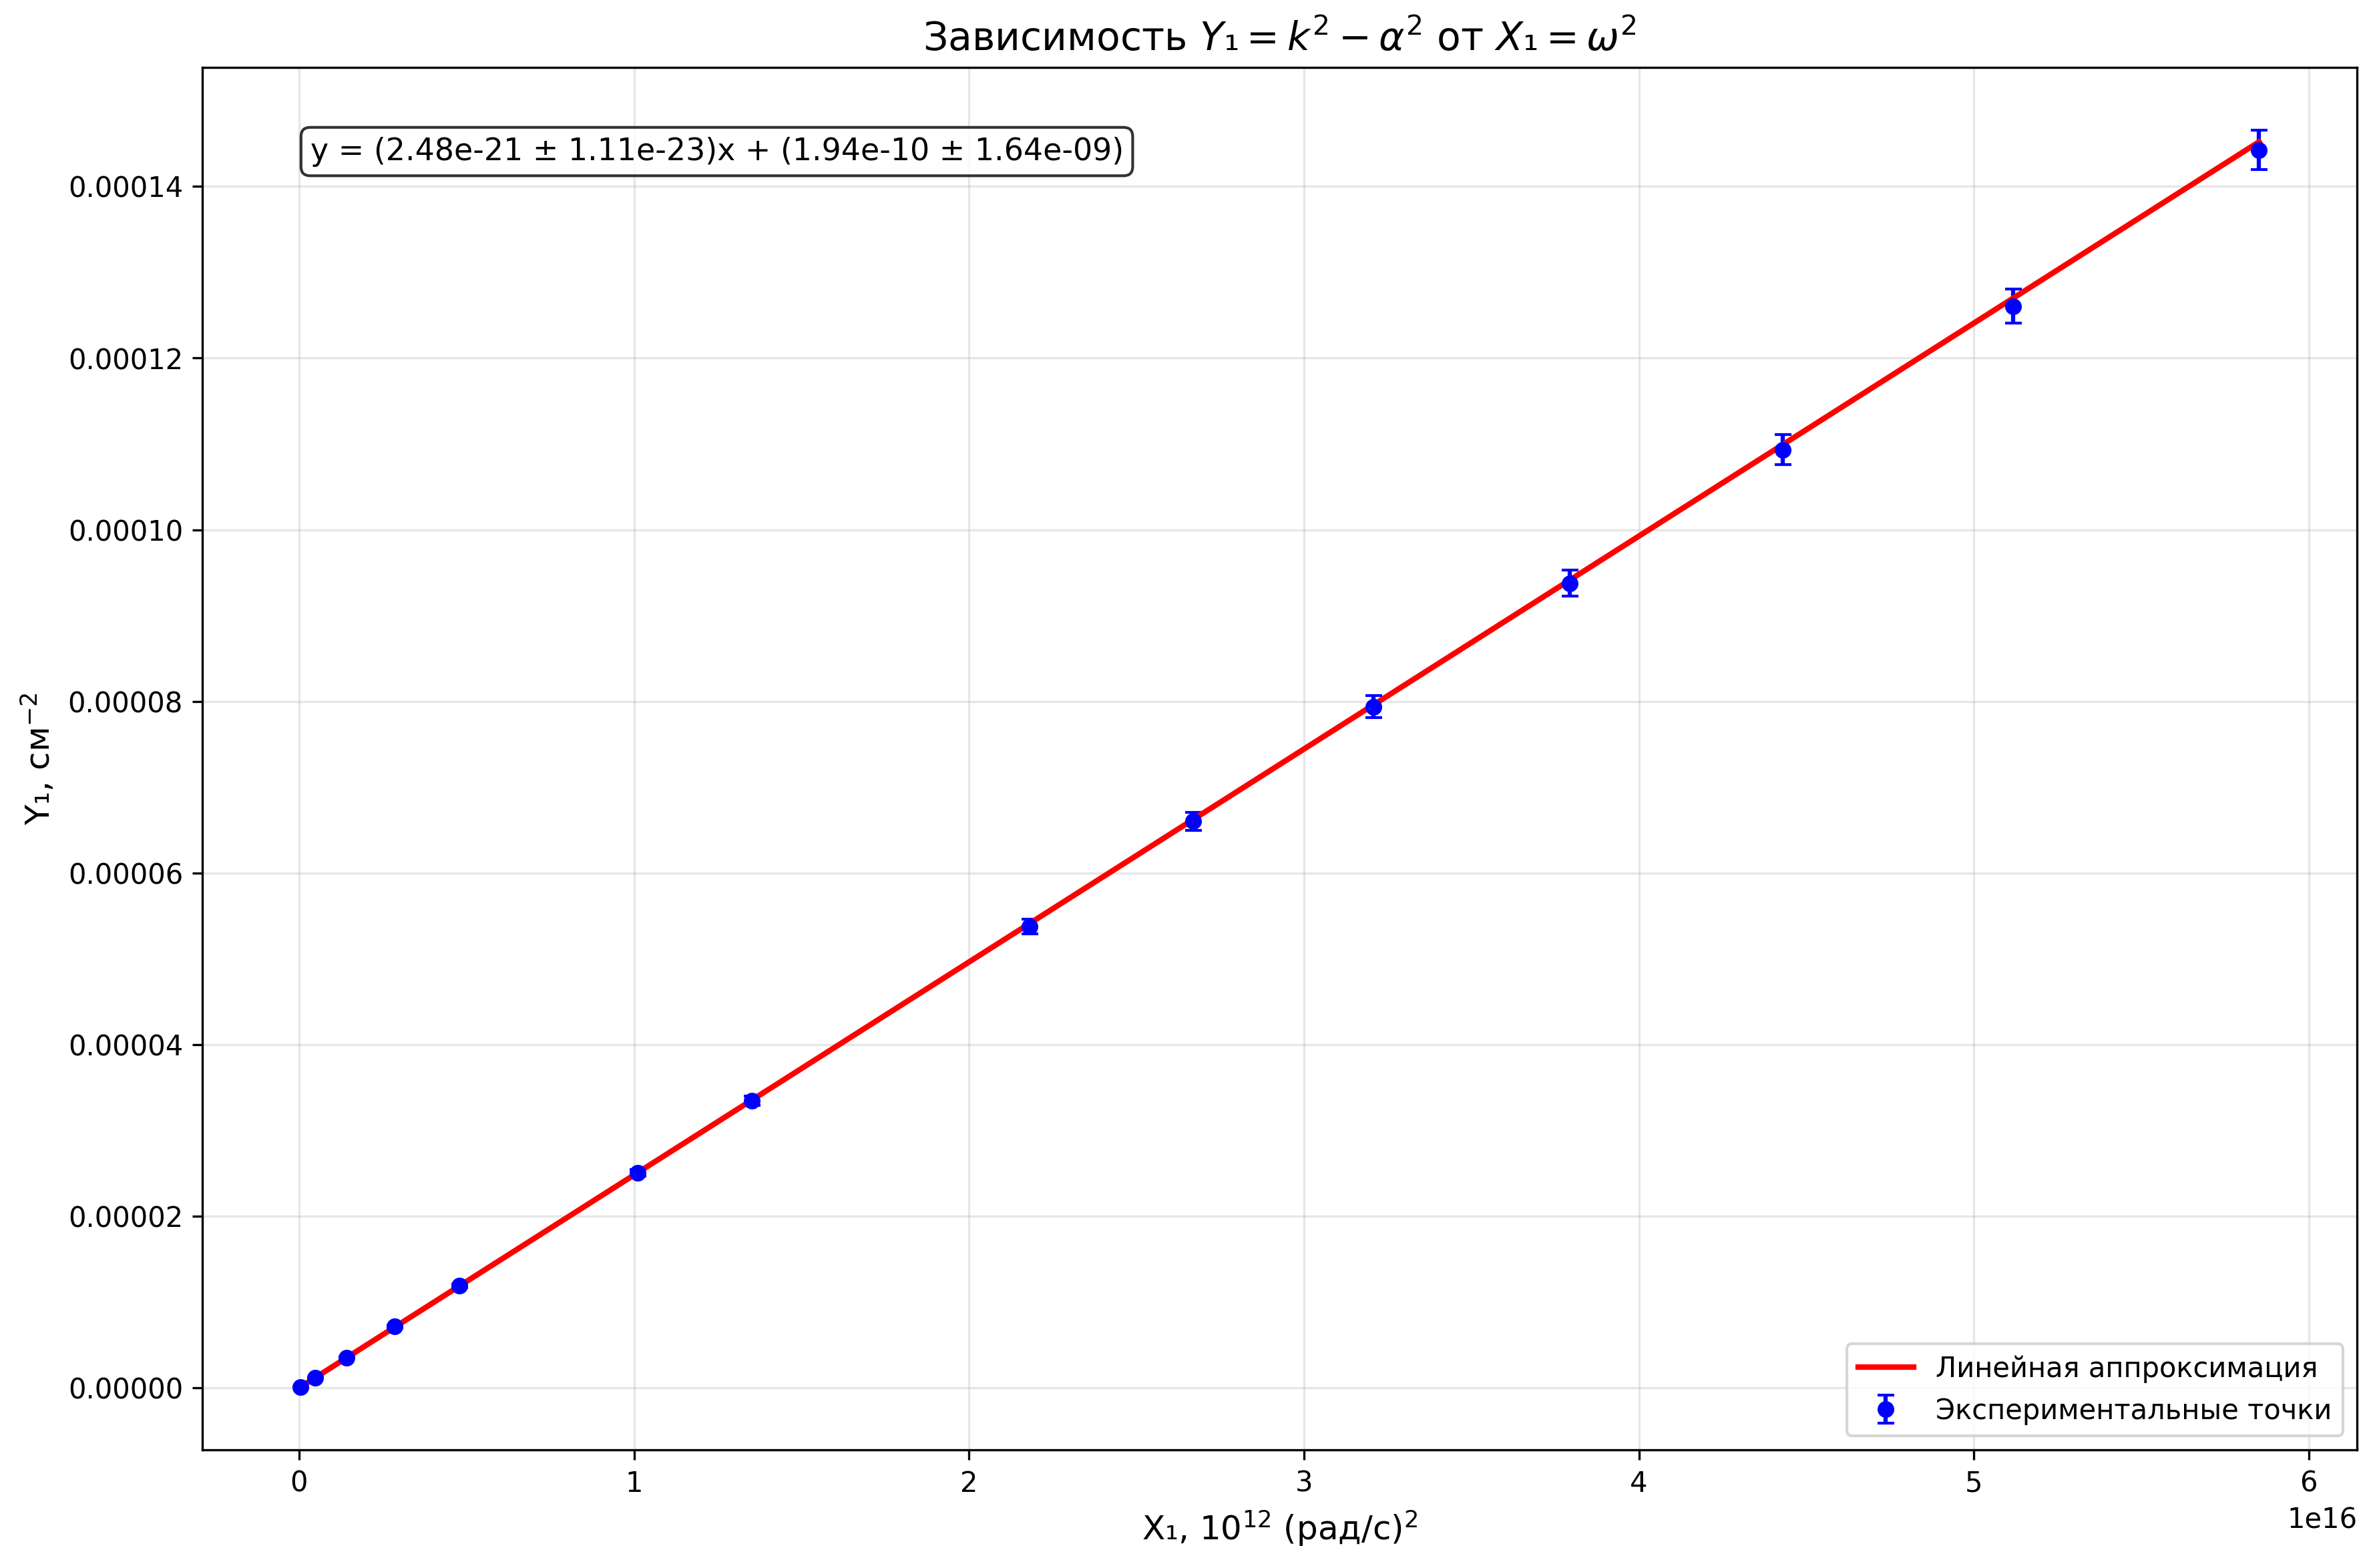
\includegraphics[width=0.85\textwidth]{Graphics/Y1_vs_X1.png}}
      \caption{График 2. Зависимость $Y_1 = k^2 - \alpha^2$ от $X_1 = \omega^2$}
\end{figure}
\clearpage
    \item Наклон графика $K_1 = (2,48 \pm 0,01) \cdot 10^{-21} \ \frac{\text{с}^2}{\text{см}^2}$ 
    \item Рассчитаем $L_x C_x = K_1 \cdot c^2 = 2,232 \pm 0,001$ 
    \item Определим погонную емкость и индуктивность кабеля. Переведем сопротивление $R_0 = 50$ ом в СГС, $R_0 = 5,56\cdot 10^{-11}$ ед. СГС. Учетом того, что $R_0 = \frac{1}{c} \sqrt{\frac{L_x}{C_x}}$, получим
\[
L_x = c R_0\sqrt{L_x C_x} = 2,493 \pm 0,006 \text{ ед. СГС} \ (\varepsilon_{L_x} = 0,22\%),
\]
\[
C_x = \frac{\sqrt{L_x C_x}}{c R_0} = 0,895 \pm 0,002 \text{ ед. СГС} \ (\varepsilon_{C_x} = 0,22\%).
\]
\item Рассчитаем диэлектрическую и магнитную проницаемости:
\[
\mu = \frac{L_x}{2 \ln{\frac{r_2}{r_1}}} = 1,029 \pm 0,022\ (\varepsilon_{\mu} = 2,17\%),
\]
\[
\varepsilon = C_x 2 \ln{\frac{r_2}{r_1}} = 2,169 \pm 0,047 \ (\varepsilon_{\varepsilon} = 2,17\%),
\]
Фазовая скорость $V_\Phi = \frac{c}{\sqrt{\mu \varepsilon}} = (2,008 \pm 0,054) \cdot 10^{10} \ \frac{\text{см}}{\text{с}}$.

Средняя взвешанная фазовая скорость по трем значениям (2 из 1-го пункта + высчитанная по проницаемостям) $V_\Phi^{\text{ср}} = (2,022 \pm 0,018) \cdot 10^{10} \ \frac{\text{см}}{\text{с}}$.

\subsubsection*{Метод А (через коэффициент затухания)}

    \item Построим по МНК график зависимости коэффициента затухания $\alpha$ от корня частоты $\sqrt{\nu}$, Проведем линейную аппроксимацию вида $\alpha = k_A \cdot \sqrt{\nu}$.
\begin{table}[h]
\centering

\begin{tabular}{|c|c|c|}
\hline
$X_2$, МГц$^{1/2}$ & $Y_2 \cdot 10^{5}$, см$^{-1}$ & $\sigma_{Y_2} \cdot 10^{5}$, см$^{-1}$ \\
\hline
1,000 & 1,512 & 5,353 \\
1,871 & 2,020 & 5,510 \\
2,449 & 2,517 & 5,587 \\
2,915 & 3,514 & 5,752 \\
3,317 & 4,207 & 5,774 \\
3,674 & 4,542 & 5,834 \\
4,000 & 4,637 & 5,938 \\
4,301 & 5,286 & 5,972 \\
4,583 & 5,886 & 6,013 \\
4,848 & 6,069 & 6,116 \\
5,099 & 6,099 & 6,233 \\
5,339 & 6,656 & 6,314 \\
5,568 & 6,986 & 6,399 \\
5,788 & 7,293 & 6,490 \\
6,000 & 7,492 & 6,634 \\
6,205 & 7,987 & 6,800 \\
\hline
\end{tabular}
\caption{Таблица 5. Данные для метода А ($\alpha$ от $\sqrt{\nu}$)}
\end{table}
\clearpage
 \begin{figure}[h]
      \center{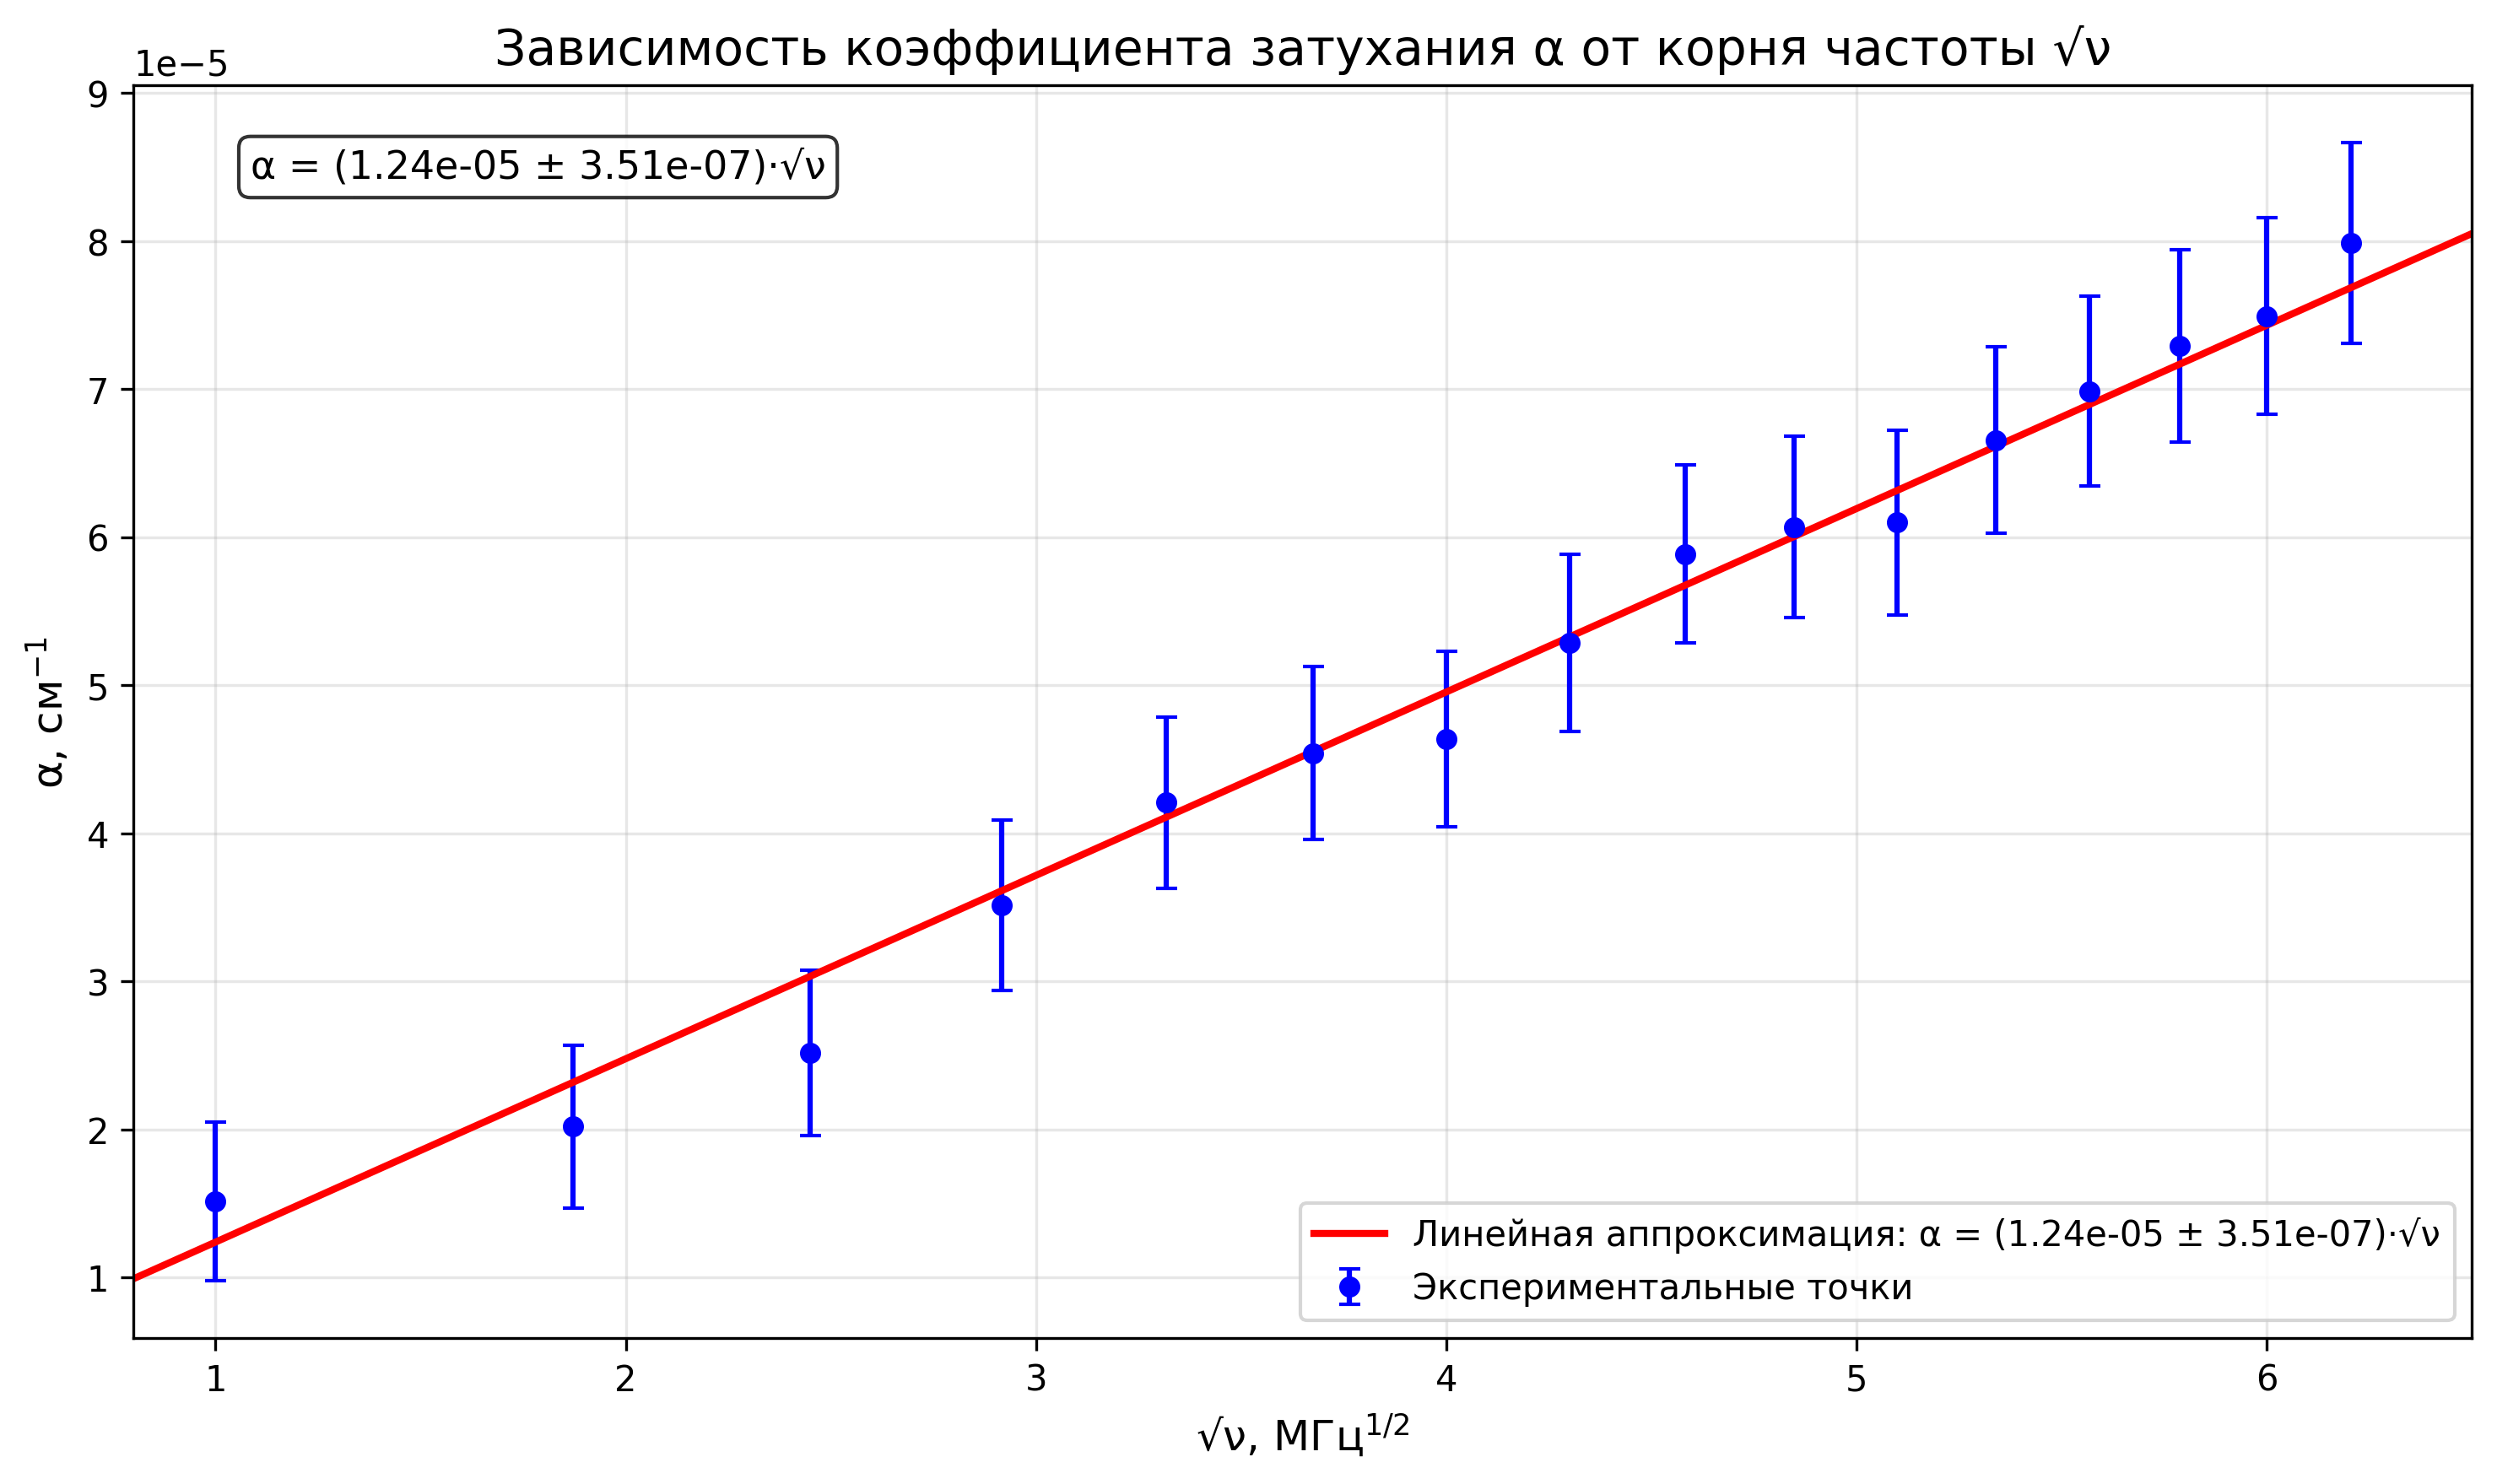
\includegraphics[width=1\textwidth]{Graphics/Y2_vs_X2.png}}
      \caption{График 3. Зависимость коэффициента затухания $\alpha$ от корня частоты $\sqrt{\nu}$}
\end{figure}
    \item Коэффициент наклона: $k_A = (1,24 \pm 0,04) \cdot 10^{-8}\ \frac{\text{см}^{-1}}{\text{Гц}^{1/2}}$ ($\varepsilon_{k_A} = 2,83 \%$).
    \item Рассчитаем удельную проводимость по формуле:
    \[
    \sigma_A = \left( \frac{4}{d} \cdot C_x \cdot \frac{V_\phi}{c} \cdot \frac{1}{k_A} \right)^2 = (2,018 \pm 0,134) \cdot 10^{18} \text{ ед. СГС} \ (\varepsilon_{\sigma_A} = 6,63\%),
    \]
    где:
    \begin{itemize}
        \item $d = 0.137$ см -- диаметр центральной жилы ($2r_1$)
        \item $C_x$ -- погонная ёмкость
        \item $V_\Phi^{\text{ср}}$ -- средняя фазовая скорость
        \item $c = 3 \cdot 10^{10}$ см/с -- скорость света
    \end{itemize}

\subsubsection*{Метод Б (через произведение $\alpha \cdot k$)}

    \item Построим график зависимости $\alpha \cdot k$ от $\nu^{3/2}$, проведем линейную аппроксимацию вида $\alpha \cdot k = k_B \cdot \nu^{3/2}$.
\clearpage
\begin{table}[h]
\centering
\begin{tabular}{|c|c|c|}
\hline
$X_3$, МГц$^{3/2}$ & $Y_3 \cdot 10^{7}$, см$^{-2}$ & $\sigma_{Y_3} \cdot 10^{7}$, см$^{-2}$ \\
\hline
1,000 & 0,474 & 1,678 \\
6,548 & 2,233 & 6,093 \\
14,697 & 4,744 & 10,54 \\
24,782 & 9,394 & 15,39 \\
36,483 & 14,51 & 19,95 \\
49,602 & 22,31 & 28,70 \\
64,000 & 23,21 & 29,78 \\
79,572 & 30,58 & 34,62 \\
96,234 & 42,01 & 43,02 \\
113,920 & 44,51 & 44,99 \\
132,575 & 49,57 & 50,81 \\
152,148 & 59,31 & 56,46 \\
172,601 & 67,65 & 62,20 \\
193,895 & 76,25 & 68,14 \\
216,000 & 84,12 & 74,78 \\
238,886 & 95,93 & 82,03 \\
\hline
\end{tabular}
\caption{Таблица 6. Данные для метода Б ($\alpha \cdot k$ от $\nu^{3/2}$)}
\end{table}

 \begin{figure}[h]
      \center{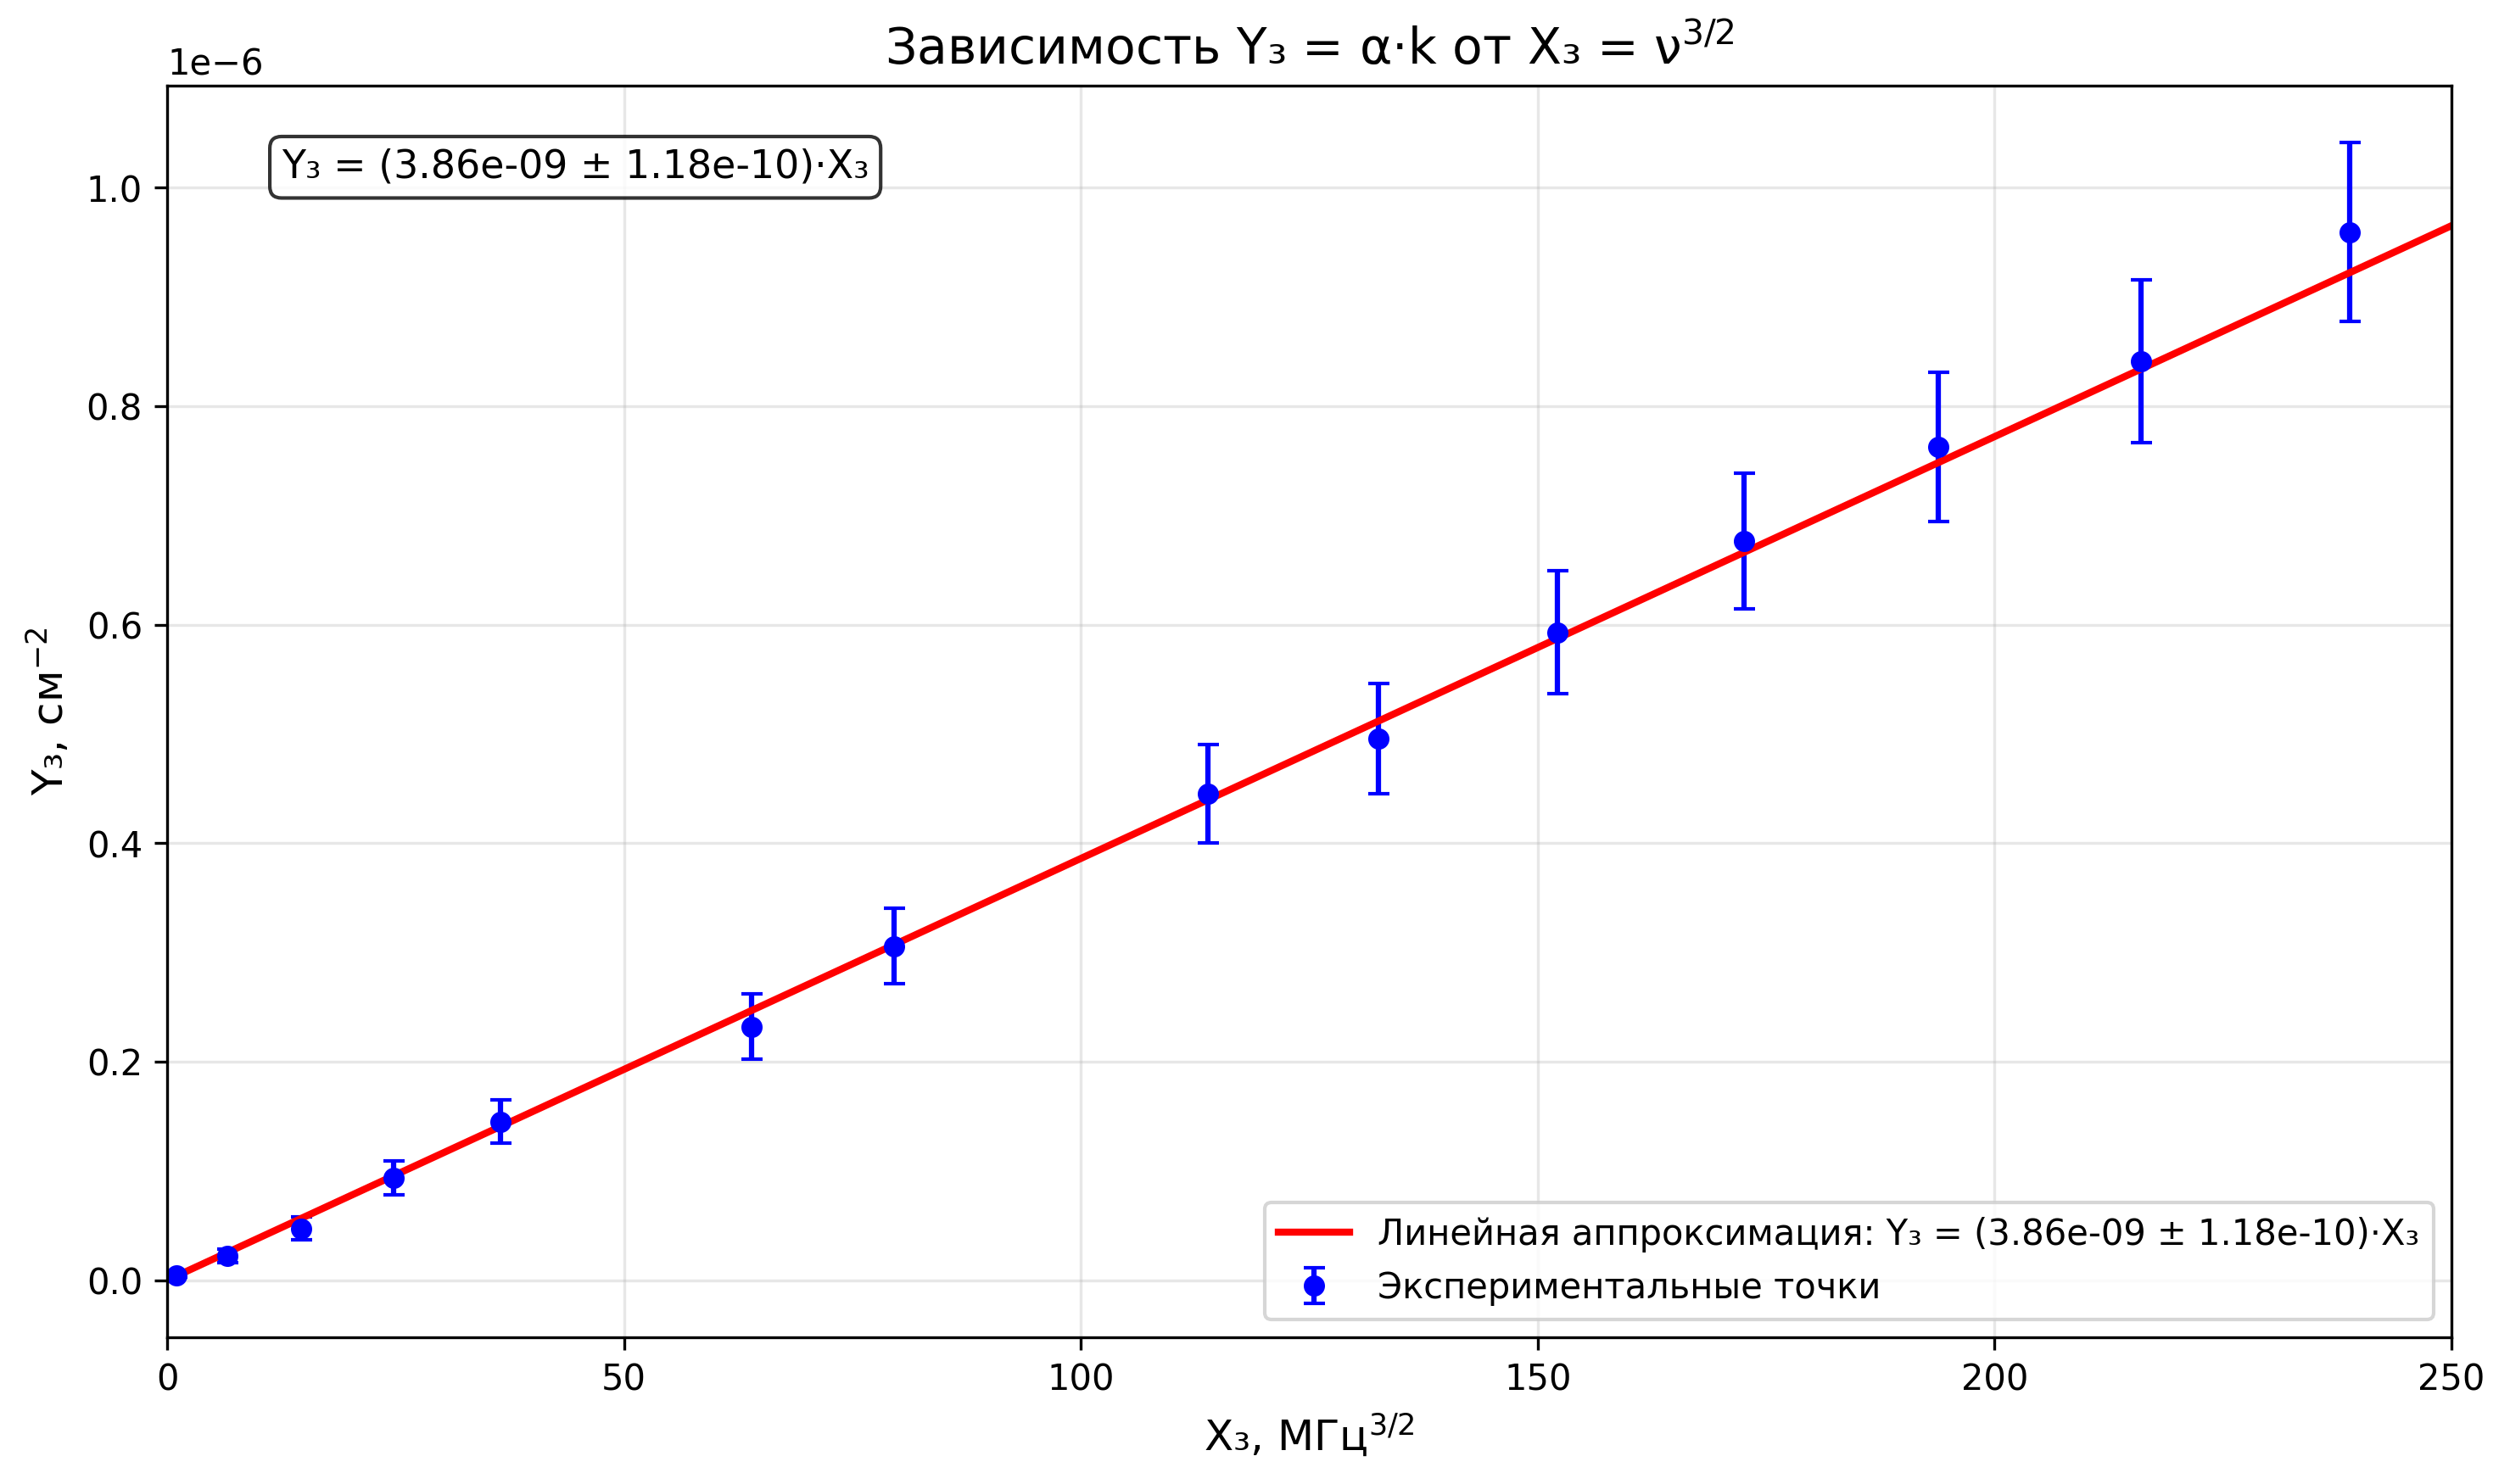
\includegraphics[width=1\textwidth]{Graphics/Y3_vs_X3.png}}
      \caption{График 4. Зависимость $\alpha \cdot k$ от $\nu^{3/2}$}
\end{figure}
    \item Коэффициент наклона: $k_B = (4.86 \pm 0.12) \cdot 10^{-8} \ \frac{\text{см}^{-2}}{\text{Гц}^{3/2}}$ ($\varepsilon_{k_\text{Б}} = 3,06 \%$).
    \item Рассчитаем удельную проводимость по формуле:
    \[
    \sigma_\text{Б} = \left( \frac{4\pi \cdot C_x}{d \cdot c \cdot k_\text{Б}} \right)^2 = (0,503 \pm 0,034) \cdot 10^{18} \text{ ед. СГС} \ (\varepsilon_{\sigma_\text{Б}} = 6,79\%),
    \]

\end{enumerate}

\section{Результаты и обсуждения}

\subsection*{Сводка полученных результатов}

В ходе эксперимента были определены основные параметры коаксиального кабеля Eltros PK 50-4-11. Все измерения проводились в системе СГС.

\begin{table}[h!]
\centering
\begin{tabular}{|c|c|c|c|}
\hline
Параметр & Значение & Погрешность & Отн. погрешность, \% \\
\hline
$L_x C_x$, ед. СГС & 2,232 & 0,001 & 0,045 \\
$L_x$, ед. СГС & 2,493 & 0,006 & 0,24 \\
$C_x$, ед. СГС & 0,895 & 0,002 & 0,22 \\
$\mu$ & 1,029 & 0,022 & 2,17 \\
$\varepsilon$ & 2,169 & 0,047 & 2,17 \\
$V_\Phi^{ср}$, $10^{10}$ см/с & 2,022 & 0,018 & 0,89 \\
$\sigma_A$, $10^{18}$ ед. СГС & 2,018 & 0,134 & 6,64 \\
$\sigma_B$, $10^{18}$ ед. СГС & 0,503 & 0,034 & 6,76 \\
\hline
\end{tabular}
\caption{Таблица 7. Сводная таблица экспериментальных результатов}
\label{tab:summary}
\end{table}

\subsection*{Сравнение с табличными значениями}

\begin{table}[h!]
\centering
\begin{tabular}{|c|c|c|c|}
\hline
Параметр & Эксперимент & Табличное значение & Расхождение \\
\hline
$\varepsilon$ (ПЭ) & 2,169 & 2,25--2,35 & 3,6--7,7\% \\
$\mu$ (медь) & 1,029 & $\approx$1,0 & 2,9\% \\
$V_\Phi/c$ & 0,674 & 0,659--0,68 & 2--4\% \\
$\sigma_A$, $10^{18}$ ед. СГС & 2,02 & 0,0537 & в 37,6 раз \\
$\sigma_B$, $10^{18}$ ед. СГС & 0,503 & 0,0537 & в 9,4 раз \\
\hline
\end{tabular}
\caption{Таблица 8. Сравнение с табличными значениями}
\label{tab:comparison}
\end{table}

\subsection*{Анализ результатов}

\textbf{Фазовая скорость и волновые параметры}. Полученное значение фазовой скорости $V_\Phi = (2,022 \pm 0,018) \cdot 10^{10}$ см/с хорошо согласуется с теоретическим предсказанием для коаксиального кабеля с полиэтиленовым заполнением. Относительная скорость $V_\Phi/c = 0,674$ соответствует диэлектрической проницаемости $\varepsilon \approx 2,2$, что характерно для полиэтилена.

\textbf{Диэлектрическая и магнитная проницаемости}. Значение $\varepsilon = 2,169$ несколько ниже табличного для полиэтилена (2,25--2,35), что может быть связано с наличием воздушных зазоров в кабеле. Значение $\mu = 1,029$ близко к 1, что ожидаемо для меди.

\textbf{Удельная проводимость}. Наблюдается значительное расхождение между экспериментальными и табличными значениями:
\begin{itemize}
\item Метод А дал значение $\sigma_A = 2,02 \cdot 10^{18}$ ед. СГС, что в 37,6 раз превышает табличное значение для меди
\item Метод Б показал $\sigma_B = 0,503 \cdot 10^{18}$ ед. СГС, что в 9,4 раз превышает табличное значение
\end{itemize}

\textbf{Возможные причины расхождений}:
\begin{enumerate}
\item Приближенный характер модели скин-слоя на используемых частотах
\item Систематические погрешности измерения амплитуд и фазовых сдвигов
\item Влияние поверхностной шероховатости проводников на высоких частотах
\item Накопление погрешностей при вычислении производных параметров
\item Отличие реальных геометрических параметров кабеля от заявленных
\end{enumerate}

\textbf{Сравнение методов}. Метод Б показал значительно лучшее согласие с табличными данными, чем метод А. Это может быть связано с тем, что метод Б использует непосредственно измеренные величины $\alpha$ и $k$ и не требует знания фазовой скорости, тогда как метод А чувствителен к точности определения $V_\Phi$.

\textbf{Качество аппроксимации}. Все построенные графики демонстрируют высокое качество линейной аппроксимации, что подтверждает адекватность использованных теоретических моделей и точность экспериментальных измерений.

\section{Вывод}

\begin{enumerate}
\item Экспериментально определены волновые параметры коаксиального кабеля: $L_x = 2,493$ ед. СГС, $C_x = 0,895$ ед. СГС, $L_x C_x = 2,232$ ед. СГС

\item Рассчитаны диэлектрическая и магнитная проницаемости: $\varepsilon = 2,169$, $\mu = 1,029$, что соответствует ожидаемым значениям для полиэтилена и меди

\item Фазовая скорость распространения сигнала в кабеле составляет $V_\Phi = (2,022 \pm 0,018) \cdot 10^{10}$ см/с ($V_\Phi/c = 0,674$)

\item Удельная проводимость материала проводников, определенная двумя методами:
\begin{itemize}
\item Метод А: $\sigma_A = (2,018 \pm 0,134) \cdot 10^{18}$ ед. СГС (расхождение с табличным в 37,6 раз)
\item Метод Б: $\sigma_B = (0,503 \pm 0,034) \cdot 10^{18}$ ед. СГС (расхождение с табличным в 9,4 раз)
\end{itemize}

\item Метод Б демонстрирует лучшее согласие с табличными данными, хотя оба метода дают завышенные значения удельной проводимости

\item Относительные погрешности измерений не превышают 7\%, что свидетельствует о хорошей воспроизводимости результатов

\item Полученные результаты подтверждают применимость телеграфных уравнений для описания распространения сигналов в коаксиальных линиях и демонстрируют влияние скин-эффекта на затухание высокочастотных сигналов

\item Для улучшения точности определения удельной проводимости рекомендуется использовать метод Б и проводить измерения на более высоких частотах, где скин-эффект выражен более явно
\end{enumerate}
\end{document}